% Pacotes
\documentclass[12pt]{article}
\usepackage{adjustbox}
\usepackage[utf8]{inputenc}
\usepackage{amsmath}
\usepackage{hyperref}
\usepackage{sbc-template}
\usepackage{fancyvrb}
\usepackage{amsfonts}
\usepackage{amsmath}
\usepackage{graphicx,url}


\sloppy

\title{Atom\\O Editor Open Source do GitHub}

\author{Ricardo Henrique Brunetto\inst{1}}


\address{Departamento de Informática -- Universidade Estadual de Maringá (UEM)\\
	Maringá -- PR -- Brasil
	\email{ra94182@uem.br}
}

\begin{document}

	\maketitle

	{\resumo{O presente trabalho visa a apresentar de forma instrutiva as funcionalidades do editor de texto Atom e tratar a respeito de suas vantagens, desvantagens, formas de instalação e recursos que o diferenciam dos demais editores. Este trabalho segue referência direta da documentação oficial do Atom \cite{doc:atom}, embora algumas seções não sejam mencionadas a fim de manter concisão.}}

	\newpage
	\tableofcontents
	\newpage

  \section{Introdução}\label{sec:intro}
	O Atom é um editor de texto de código aberto desenvolvido pelo GitHub e liberado como beta em junho de 2015 sob a Licença MIT \cite{licencaMIT}, projetado para combinar flexibilidade e extensibilidade. De forma geral, o Atom é um editor focado em desenvolvimento de código, oferecendo recursos e ferramentas para solucionar dos mais ínfimos aos mais significativos inconvenientes do ofício. Além disso, por ser um software livre e aberto e fornecer suporte à extensões criadas pelos própriros usuários, o Atom passou a ser conhecido como "Editor de Texto Hackeável do Século 21".

	O Atom foi desenvolvido através do Electron e de outras tecnologias web (HTML, Javascript e CSS). O ponto-chave do Atom como editor de texto é um compromisso com a hackeabilidade e usabilidade, o que significa que os principais avanços e diferenciais do software se concentram em proporcionar ao usuário uma forma de personalizar por completo sua experiência. Dessa forma, o usuário consegue criar \textit{plug-ins} e extensões conforme sua necessidade e propósito.

	Dessa forma, o Atom é composto por seu núcleo, ferramentas e componentes que são adotados como oficiais e vêm instalados (bem como o próprio editor), e pelos \textit{add-ons} desenvolvidos pelos próprios usuários e disponíveis em repositórios na web (em especial no GitHub). A respeito do núcleo do Atom, alguns aspectos são interessantes e passíveis de abordagem.

	Duas décadas de desenvolvimento Web permitiram que a mesma evoluísse para uma incrível e poderosa plataforma. Contudo, codificar é uma tarefa especial que requer ferramentas dedicadas. Por isso, o Atom não foi escrito como uma aplicação web tradicional, mas sim como uma variante específica do Chromium, dedicada à escrita de texto.

	Abrindo um rápido parênteses, o Chromium é um conjunto de projetos que incluem um navegador web de código aberto e livre que a Google usa como base para o desenvolvimento do Google Chrome, e um sistema operacional onde a Google também se baseia para o Chrome OS. Mais informações podem ser encontradas em \cite{doc:chromium}.

	Outro grande benefício é garantir que tudo está rodando na mais nova versão do Chromium. Isso significa que não há preocupações em relação à compatibilidade ou versionamentos. Dessa forma, os mais recentes recursos e frameworks desenvolvidos na Web para uso em aplicações podem ser incluídos no Atom sem que haja problemas de compatibilidade com projetos já em desenvolvimento.

	Desenvolver um editor de texto baseado em tecnologias Web é um acerto no sentido em que se tem grande capacidade de crescimento, visto que, embora as tecnolgias nativas variem entre si, as tecnologias Web permanecem por serem multi-plataforma e irrestritas quanto às possiblidades de desenvolvimento.

	De acordo com os próprios desenvolvedores, o Atom exerce um papel complementar à função do GitHub de proporcionar software melhor através do trabalho em equipe, o que implica que o editor é, na verdade, um investimento à longo prazo, sempre respaldado pelo suporte do próprio GitHub. Além disso, conforme outros editores como Emacs e Vim demonstraram com o passar dos anos, o desenvolvimento de um software estável, de grande comunidade e eficiente, necessita ter código aberto.

	\section{Instalação}\label{sec:inst}
	Disponível nos sitemas operacionais Mac, Windows e Linux, instalar o Atom é realmente simples, em todos eles. O primeiro passo é fazer o \textit{download} da versão compatível com o sistema operacional em \href{https://atom.io}{https://atom.io}.

	A seguir serão explorados detalhes particulares da instação do Atom em cada um dos sistemas operacionais em que está disponível.

	\subsection{Instalação no Windows}\label{sec:instwin}
	Dentre as opções de \textit{download} mencionadas acima, há uma versão com o \textit{Windows Installer}. Após realizar a instalação seguindo as instruções do instalador, será instalado o Atom,bem como seus atalhos na área de trabalho e menu de inicialização, e serão adicionados os comandos \verb|atom| e \verb|apm| na variável do sistema \verb|PATH|, para que também se possa manipular o programa por linha de comando através do terminal (no Windows, \verb|cmd|).

	Além disso, as opções \verb|Abrir com Atom| e as associações em \verb|Abrir com...| serão criadas automaticamente. Contudo, isso pode ser controlado através de um painel no próprio Atom. Basta acessar o menu \verb|File > Settings| e escolher \verb|System| no painel lateral. Em ordem, de acordo com a Figura \ref{fig:fig1}, as opções: Registra o Atom no menu de associação de arquivos (\verb|Abrir com...|); Mostra a opção \verb|Abrir com Atom| no menu de contexto de arquivos; Mostra a opção \verb|Abrir com Atom| no menu superior do Explorer.

	\begin{figure}[h]
		\centering
		\label{fig:fig1}
		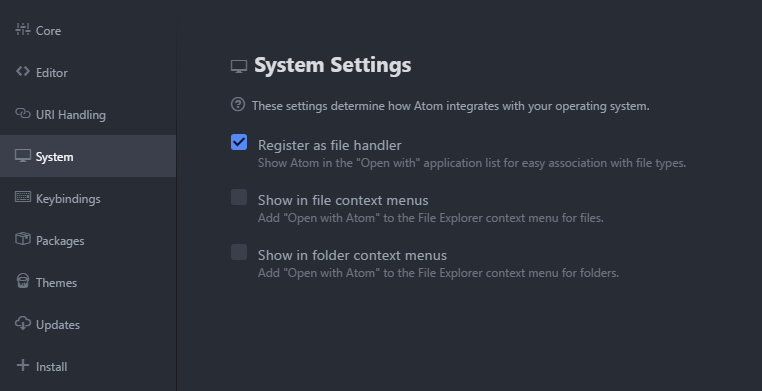
\includegraphics[scale = 0.7]{fig1}
		\caption{Menu de controle das opções do Sistema no Windows.}
	\end{figure}

	\subsubsection{Modo Portátil}\label{sec:portable}
	O Atom possui um Modo Portátil (\textit{Portable Mode}) disponível para ser utilizado.

	As configurações e estados do Atom são armazenados em \textit{\%userprofile\%$\backslash$.atom} (no Windows, \textit{\%userprofile\%} por padãro referencia \textit{C:$\backslash$users$\backslash$NOME\_DE\_USUARIO}). Assim, o usuário pode executar o Atom com modo portátil onde o programa e suas configurações estão armazenados juntos, tal como em um dispositivo de armazenamento removível (\textit{ex: pendrives}).

	Para configurar o modo portátil, basta fazer o download da versão correspondente ao sistema operacional em \href{https://github.com/atom/atom/releases/latest}{https://github.com/atom/atom/releases/latest} e extrair no dispositivo de armazenamento removível. Após isso, crie uma pasta intitulada \textit{.atom} no mesmo diretório que contém a pasta extraída. Por exemplo, se a extração foi realizada em \textit{E:$\backslash$}, então deve-se ter:
	\begin{Verbatim}[fontsize=\footnotesize]
		E:\atom-1.14\atom.exe
		E:\.atom
	\end{Verbatim}
	Algumas observações em relação ao Modo Portátil são válidas:
	\begin{enumerate}
		\item O diretório \textit{.atom} deve ser gravável (\textit{writable});
		\item Não é necessário criar a pasta \textit{.atom}. Pode-se copiar uma já existente;
		\item O Atom pode armazenar configurações de usuário do Electron na pasta \textit{electronUserData};
		\item Tambem é possível criar uma variável de ambiente \verb|ATOM_HOME| para referenciar o diretório \textit{.atom} ou um script (\textit{.sh, .cmd}) para inicializá-lo;
		\item A instação em Modo Portátil \textbf{não} atualizará automaticamente.
	\end{enumerate}

	\subsubsection{Configurações de Firewall e Proxy}\label{sec:fireproxy}
	Em caso de problemas com o Firewall ou erros de SSL ao instalar os pacotes, pode-se desativar a opção de rigorosidade do SSL através do prompt de comando do (no Windows: \verb|[Win + R] > cmd > [ENTER]|) com a seguinte linha de comando:
	\begin{Verbatim}[fontsize=\footnotesize]
		apm config set strict-ssl false
	\end{Verbatim}

	Caso o problema seja em relação ao Proxy, pode-se configurar um proxy HTTP(S) através da seguinte linha de comando:
	\begin{Verbatim}[fontsize=\footnotesize]
		apm config set https-proxy SEU_ENDERECO_PROXY
	\end{Verbatim}
	onde \verb|SEU_ENDERECO_PROXY| é o endereço de proxy a ser utilizado.

	\subsection{Mac}
	De forma semelhante à instalação no Windows (vide Seção \ref{sec:instwin}), a instação do Atom segue o padrão do sistema operacional. Nesse caso, o padrão zip para as instalações no Mac. O \textit{download} pode ser feito alternativamente em \href{https://github.com/atom/atom/releases/latest}{https://github.com/atom/atom/releases/latest} através do arquivo \textit{atom-mac.zip}. Após baixar o arquivo, basta extraí-lo e arrastar o \verb|Atom| para a pasta \textit{Aplicações} (ou \textit{Applications}).

	Ao abrir a aplicação pela primeira vez, os comandos \verb|atom| e \verb|apm| serão instalados. Em alguns casos, o Atom pode não conseguir realizar esta etapa, visto que pode ser necessária a senha do adminstrador. Para verificar se houove sucesso, basta abrir o terminal de comando do Mac e inserir a linha de comando \verb|which atom|. Em caso de sucesso, será retornado o local de instalação (em geral, \verb|/usr/local/bin/atom|) e, caso contrário, nada será retornado.

	Uma nova tentativa de instalação dos comandos pode ser feita na Paleta de Comandos (\textit{Command Palette}) do Atom (explanada na Seção \ref{sec:commandpalette}) através do seguinte comando: \verb|Window: Install Shell Commands|.

	\subsubsection{Modo Portátil}
	As configurações de instalação e as observações válidas são exatamente como mencionado na Seção \ref{sec:portable}. As diferenças, contudo, estão na forma como os arquivos são organizados. No Mac, a hierarquia das pastas para a configuração do modo portátil (\textit{.atom}) seria:
	\begin{Verbatim}[fontsize=\footnotesize]
		/MyUSB/Atom.app
		/MyUSB/.atom
	\end{Verbatim}

	Além disso, as configurações e estados do Atom \textbf{não} são armazenados em \textit{\%userprofile\%$\backslash$.atom} pois o Mac não fornece uma variável \textit{\%userprofile\%}, sendo tais configurações armazenadas na pasta \textit{home} do usuário.

	\subsubsection{Configurações de Firewall e Proxy}
	Em caso de problemas com Firewall ou Proxy, basta seguir as instruções da Seção	\ref{sec:fireproxy}, pois os comandos (e suas sintaxes) são idênticos nos sistemas operacionais disponíveis.

	\subsection{Linux}
	No Linux, pode-se utilizar o Gerenciador de Pacotes (\textit{Package Manager}) para configurar um dos repositórios oficiais do Atom, o que também permtirá atualizar o Atom quando possível.

	A seguir, serão explanados detalhes para as principais distribuições do Linux onde o Atom está presente. Vale salientar que, para distribuições baseadas nas apresentadas, pode-se seguir as mesmas instruções. \textbf{Todas} as instruções a seguir são realizadas em linha de comando do \textbf{Terminal} do Linux. Não é utilizado o recurso gráfico dos sistemas operacionais para tal. Além disso, todos os comandos que incluirem \verb|sudo| podem requerer senha de administrador.

	\subsubsection{Debian e Ubuntu (deb/apt)}
	Inicialmente, adicionam-se os repositórios oficiais para o Gerenciador de Pacotes das distribuições através das seguintes linhas de comando:
	\begin{Verbatim}[fontsize=\footnotesize]
$ curl -L https://packagecloud.io/AtomEditor/atom/gpgkey | sudo apt-key add -
$ sudo sh -c 'echo "deb [arch=amd64] \
	https://packagecloud.io/AtomEditor/atom/any/ any main" > \
	/etc/apt/sources.list.d/atom.list'
$ sudo apt-get update
	\end{Verbatim}

	Após atualizar os repositórios, instala-se o Atom através do comando \verb|apt-get|:
	\begin{Verbatim}[fontsize=\footnotesize]
$ sudo apt-get install atom
	\end{Verbatim}
	Ou, para instalar o Atom versão Beta:
	\begin{Verbatim}[fontsize=\footnotesize]
$ sudo apt-get install atom-beta
	\end{Verbatim}

	Alternativamente, pode-se instalar o Atom através do pacote \textit{.deb}:
	\begin{Verbatim}[fontsize=\footnotesize]
$ sudo dpkg -i atom-amd64.deb
$ sudo apt-get -f install
	\end{Verbatim}
	onde a segunda linha serve para instalar as dependências do Atom, caso estejam faltando.

	\subsubsection{Red Hat e CentOS ou Fedora}
	Aqui ocorrem dois casos diferentes, uma vez que as distribuições Red Hat e CentOS (e suas derivadas) fazem uso do comando \verb|yum| para instalações, em face ao comando \verb|dnf| usado pelo Fedora e suas derivações.

	Partindo do mesmo princípio, adicionam-se inicialmente os repositórios oficiais do Atom no Gerenciador de Pacotes:
	\begin{Verbatim}[fontsize=\footnotesize]
$ sudo rpm --import https://packagecloud.io/AtomEditor/atom/gpgkey
$ sudo sh -c 'echo -e "[Atom]\nname=Atom \
  Editor\nbaseurl=https://packagecloud.io/AtomEditor/atom/el/7/ \
  \$basearch\nenabled=1\ngpgcheck=0\nrepo_gpgcheck=1 \
  \ngpgkey=https://packagecloud.io/AtomEditor/atom/gpgkey" > \
  /etc/yum.repos.d/atom.repo'
	\end{Verbatim}

	Neste momento, instala-se o Atom através da linha de comando:
	\begin{itemize}
		\item Red Hat / CentOS
		\begin{Verbatim}[fontsize=\footnotesize]
	$ sudo yum install atom
	$ sudo yum install atom-beta
		\end{Verbatim}
		\item Fedora
		\begin{Verbatim}[fontsize=\footnotesize]
	$ sudo dnf install atom
	$ sudo dnf install atom-beta
		\end{Verbatim}
	\end{itemize}

	\subsubsection{Modo Portátil}
	As configurações de instalação e as observações válidas são exatamente como mencionado na Seção \ref{sec:portable}. As diferenças, contudo, estão na forma como os arquivos são organizados. No Linux, a hierarquia das pastas para a configuração do modo portátil (\textit{.atom}) seria:
	\begin{Verbatim}[fontsize=\footnotesize]
		/media/myusb/atom-1.14/atom
		/media/myusb/.atom
	\end{Verbatim}

	Além disso, as configurações e estados do Atom \textbf{não} são armazenados em \textit{\%userprofile\%$\backslash$.atom} pois as distribuições do Linux não fornecem uma variável \textit{\%userprofile\%}, sendo tais configurações armazenadas na pasta \textit{home} do usuário.

	\subsubsection{Configurações de Firewall e Proxy}
	Em caso de problemas com Firewall ou Proxy, basta seguir as instruções da Seção	\ref{sec:fireproxy}, pois os comandos (e suas sintaxes) são idênticos nos sistemas operacionais disponíveis.

	\subsection{Construindo do Código-Fonte}
	Além de baixar o instalador, também é possível compilar diretamente o código-fonte nos sistemas operacionais Mac, Windows, Linux e FreeBSD.

	Os detalhes de como fazer isso estão disponíveis na Seção \ref{sec:hackingcore}.

	\section{Uso do Atom}
	Aqui serão explorados alguns detalhes a respeito da utilização do Atom. A Seção iniciar-se-á com um manual básico de utilização e, posteriormente, explorará as funções do editor que podem ser utilizadas pelo usuário. Algumas destas funções foram comentadas na Seção \ref{sec:intro}.

	\subsection{Básico}
	Aqui são exploradas as configurações e recursos básicos do Atom.

	\subsubsection{Paleta de Comandos}\label{sec:commandpalette}
	A Paleta de Comandos pode ser acessada através do menu superior em \verb|View > Toggle Command Palette| ou pelo atralho de teclas padrão: \verb|Ctrl + Shift + P| no Windows e no Linux; ou \verb|Cmd + Shift + P|, no Mac.

	Em resumo, a Paleta de Comandos é um menu guiado por buscas. Nele, pode-se encontrar quaisquer tarefas que são possíveis de serem realizadas no Atom. Serve, principalmente, para evitar a busca exaustiva em todos os menus para encontrar determinada funcionalidade, conforme ilustra a Figura \ref{fig:paleta}.

	\begin{figure}[h]
		\centering
		\label{fig:paleta}
		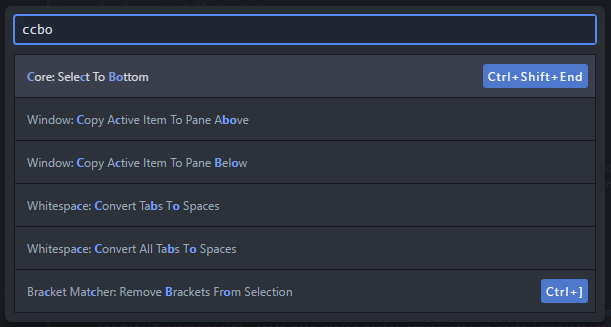
\includegraphics[scale = 0.7]{paleta}
		\caption{Paleta de Comandos do Atom no Windows.}
	\end{figure}

	A busca na Paleta de Comandos é extremamente eficiente, uma vez que faz uso de uma expressão regular baseada unicamente na ordem dos caracteres inseridos. Além de encontrar os comandos, o menu da paleta também exibe os atalhos de tecla associados a eles. Mais da Paleta de Comandos será explorada durante este artigo.

	\subsubsection{Configurações e Preferências}\label{sec:settings}
	No Atom, as Configurações e Preferências podem ser modificadas no Painel (costumeiramente referenciado na literatura como \textit{View}) de Configurações. As opções variam entre a troca de tema, quebras de linha, tamanho da tabulação, velocidade do \textit{scroll} e gerenciamento de pacotes (\textit{Packages}, a ser tratado na Seção \ref{sec:packages}).

	Cabe salientar que essas informações são mantidas na pasta \textit{.atom}.

	O acesso ao Painel de Configurações do Atom pode se dar de diferentes maneiras:
	\begin{itemize}
		\item No menu superior, \verb|File > Settings|
		\item Na Paleta de Comandos, \verb|settings-view:open|
		\item Pelo atalho de teclas padrão \verb|Ctrl + ,|
	\end{itemize}

	No Painel de Configurações, existem outros paineis anexados, conforme se nota no menu lateral. As opções permitem visualizar categorias específicas das configurações, o que facilita ao usuário encontrar a alteração que deseja realizar.

	Neste menu também é possível encontrar a opção para alterar os temas do Atom (vide Seção \ref{sec:packages}). Por padrão, o Atom possui quatro diferentes temas de Interface Gráfica, claras e escuras, bem como oito temas diferentes para sintaxe. Os temas de Interface Gráfica controlam elementos como as abas e menus, enquanto os temas de Sintaxe modificam o destaque de sintaxe (\textit{syntax highlighting}). Além disso, há a possibilidade do usuário baixar um tema pronto do repositório do Atom em \href{https://atom.io}{https://atom.io}, customizar um tema já existente (mais informações em \href{http://flight-manual.atom.io/using-atom/sections/basic-customization/}{http://flight-manual.atom.io/using-atom/sections/basic-customization/}) ou criar seu próprio tema (mais informações em \href{http://flight-manual.atom.io/hacking-atom/sections/creating-a-theme/}{http://flight-manual.atom.io/hacking-atom/sections/creating-a-theme/}).

	Outro recurso interessante que pode ser encontrado neste Painel é a quebra de linha automática. Isso é particularmente útil ao fazer do Atom um editor de documentos (principalmente em \LaTeX). O recurso está disponível neste mesmo Painel de Configurações, permitindo inclusive substituir espaços por tabulações e vice-versa.

	\subsubsection{Pastas de Projeto}
	O Atom possui uma estrutura chamada de Árvore de Visualização (\textit{Tree View}), por padrão anexada ao menu lateral esquerdo, onde o usuário pode visualizar toda a hierarquia de diretórios e arquivos que está manipulando, o que permite navegar com facilidade entre os mesmos para que sejam editados com um único clique. Pode-se alternar a exibição da Árvore com \verb|Ctrl + \| e focar através de \verb|Alt + \|. Quando a Árvore possui foco, pode-se pressionar \verb|A| para adicionar um arquivo, \verb|M| para movê-lo e \verb|Delete| para deletá-lo.

	Para adicionar uma Pasta de Projeto (\textit{Project Folder}) e, desse modo, constar na Árvore de Visualização, pode-se utilizar o menu superior em \verb|File > Add Project Folder| ou usar o atalho padrão \verb|Ctrl + Shift + A| e navegar até a pasta desejada. Alternativamente, por linha de comando (em todos os Sistemas Operacionais), pode-se utilizar:
	\begin{Verbatim}[fontsize=\footnotesize]
$ atom <lista-de-diretorios>
	\end{Verbatim}
	onde \verb|<lista-de-diretorios>| é a sequência de diretórios a serem concebidos como Pasta de Projeto no Atom, separados por espaço.

	O Atom também suporta facilidades em relação à busca de arquivos. Dada uma pasta de projeto que esteja selecionada, o usuário pode pressionar \verb|Ctrl + T| ou \verb|Ctrl + P| e buscar pelo nome do arquivo (funcionalidade chamada de \textit{Fuzzy Finder}) desejado, em uma sintaxe de busca semelhante à explanada na Seção \ref{sec:commandpalette}, com a busca pela Paleta de Comandos. Além disso, existem parâmetros para filtrar a busca de acordo com o tipo de arquivo e iniciam com "." após a \textit{string} de busca. A lista destes parâmetros pode ser contrada aqui:  \href{http://flight-manual.atom.io/getting-started/sections/atom-basics/}{http://flight-manual.atom.io/getting-started/sections/atom-basics/}.

	\subsection{Packages}\label{sec:packages}
	O Atom por si próprio é constituído de um núcleo base composto por um determinado número de pacotes (\textit{packages}) e uma funcionalidade capaz de adicionar outros. O \textit{Fuzzy Finder}, a tela de boas vindas, os temas, a Árvore de Visualização, o Painel de Configurações, são todos pacotes independentes que são mantidos por APIs e servem ao Atom.

	Isso implica que existem muitas outras funcionalidades passíveis de serem desenvolvidas por quaisquer usuário e disponibilizadas nos repositórios do GitHub. Para instalar novos pacotes, basta acessar o Painel de Configurações (vide Seção \ref{sec:settings}), clicar em \textit{Install} no menu lateral esquerdo, e verificar as opções disponíveis.

	Os pacotes listados são disponibilizados em \href{https://atom.io/packages}{https://atom.io/packages}, que é o repositório oficial de pacotes do Atom.

	Todos os pacotes instalados podem ser desabilitados ou desinstalados de acordo com a necessidade do usuário. Ao acessar as configurações de um pactoe, pode-se visualizar as opções relacionadas, desde atualização, configurações particulares do pacote, versionamento e código-fonte.

	Pode-se também instalar temas a partir do Painel de Configurações, conforme já abordado na Seção \ref{sec:settings}. Pode-se, então, pesquisar pelo nome dos temas correspondentes para que então se tenha uma lista de todos os temas disponíveis no repositório oficial.

	\subsubsection{Linha de Comando}
	Pode-se instalar pacotes através da linha de comando, utilizando o comando \textit{atm}, instalado junto com o Atom, conforme descrito na Seção \ref{sec:inst}.

	Para realizar a instalação de determinado pacote, basta utilizar a seguinte sintaxe de comando:
	\begin{Verbatim}[fontsize=\footnotesize]
$ apm install <package_name>
	\end{Verbatim}
	para instalar a versão mais recente do pacote ou
	\begin{Verbatim}[fontsize=\footnotesize]
$ apm install <package_name>@<package_version>
	\end{Verbatim}
	para instalar uma versão específica.

	Pode-se, inclusive, utilizar o \verb|atm| para encontrar pacotes e, posteriormente, instalá-los, através do comando:
	\begin{Verbatim}[fontsize=\footnotesize]
$ apm search <termo>
	\end{Verbatim}
	Ou, ainda, utilizar
	\begin{Verbatim}[fontsize=\footnotesize]
$ apm view <package_name>
	\end{Verbatim}
	para obter mais detalhes sobre um determinado pacote.

	\subsection{Navegação no Atom}
	Além de fazer uso do convencional clique de mouse e setas para se locomover dentro dos arquivos, o Atom fornece uma forma prática através de atalhos do teclado, a fim de manter o usuário exclusivamente no teclado e tornar o trabalho mais rápido.

	O Atom suporta todos os atalhos padrão das teclas do Windows, Linux e Mac para locomoção em arquivos com \textit{scroll} (ex: \verb|Ctrl + End| para ir para o fim da página). Esses atalhos universais dentro do sistema operacional permanecem funcionais no Atom.

	Pode-se mover para uma específica linha ou coluna do arquivo através do atalho \verb|Ctrl + G| e inserindo as posições de acordo com a sintaxe \verb|linha| ou \verb|linha:coluna|.

	O Atom também permite que se navegue pelo arquivo através de símbolos (funções ou definições), de forma intuitíva através do Painel de Símbolos (\textit{Symbols View}), acessível através do atalho \verb|Ctrl + R| (Windows e Linux) ou \verb|Cmd + R| (Mac). Este painel exibe uma lista de todos os símbolos no arquivo atual. A partir deste painel pode-se acessar um filtro de similaridade através de \verb|Ctrl + T| (Windows e Linux) ou \verb|Cmd + T|.

	Pode-se também fazer uso de \textit{tags} para localização no arquivo, mas isso requer que se gere as tags através do pacote \verb|ctags|, cujas informações podem ser encontradas em \href{https://ctags.io/}{https://ctags.io/}.

	Além disso, o Atom possui nativamente um pacote denominado \verb|bookmarks|, que permite que o usuário faça uma marcação (denominada \textit{bookmark}) em determinada linha e avance para lá de forma rápida e prática. Em ordem:
	\begin{itemize}
		\item \verb|Alt + Ctrl + F2| adiciona um \textit{bookmark} (ou remove, caso já exista) na linha atual;
		\subitem \verb|Cmd + F2|, no Mac.
		\item \verb|F2| avança para o próximo \textit{bookmark};
		\item \verb|Shift + F2| permite navegar ciclicamente entre os \textit{bookmarks};
		\item \verb|Ctrl + F2| exibe uma lista com os \textit{bookmarks} atuais, permitindo que usuário se dirija a qualquer um.
	\end{itemize}

	\subsection{Edições no Atom}
	Existem alguns recursos fundamentais que fazem do Atom um excelente utilitário para manipular quaisquer tipos de arquivos de texto. Dentre estes recursos, está um conjunto de combinações de tecla que permitem fazer alterações em grande escala de forma rápida e prática.

	\subsubsection{Básico}
	Algumas manipulações são básicas e não são recursos exclusivos do Atom como editor de texto e executam operações essenciais:
	\begin{itemize}
		\item \verb|Ctrl + J| (ou \verb|Cmd + J| no Mac): insere a linha abaixo no final da linha atual;
		\item \verb|Ctrl + Up/Down| (ou \verb|Cmd + Up/Down| no Mac): move a linha atual para cima/baixo;
		\item \verb|Ctrl + Shift + D| (ou \verb|Cmd + Shift + D| no Mac): duplica a linha atual;
		\item \verb|Ctrl + U| (ou \verb|Cmd + U| no Mac): transforma a palavra atual apenas em letras maiúsculas \textit{Upper case};
		\item \verb|Ctrl + L| (ou \verb|Cmd + L| no Mac): transforma a palavra atual apenas em letras minúsculas \textit{Lower case};
		\item \verb|Ctrl + T| (apenas no Mac): transpõe caracteres, trocando os dois caracteres de cada lado do cursor;
		\item \verb|Ctrl + Shift + K|: exclui a linha atual;
		\item \verb|Ctrl + Backspace| (ou \verb|Alt + Backspace| no Mac): deleta até o início da palavra atual;
		\item \verb|Ctrl + Delete| (ou \verb|Alt + Delete| no Mac): deleta até o fim da palavra atual;
	\end{itemize}

	\subsubsection{Múltilplos Cursores}
	Um recurso interessante no Atom que, apesar de estar presente em outros editores de texto não é tão bem aproveitado, é a possibilidade de utilizar múltilplos cursores de texto para editar o arquivo. A praticidade oferecida por este recurso torna o Atom flexível para editar quaisquer arquivos de texto.
	\begin{itemize}
		\item \verb|Ctrl + Clique| (ou \verb|Cmd + Clique| no Mac): Adiciona um novo cursor na posição do clique;
		\item \verb|Ctrl + Alt + Up/Down| ou (\verb|Ctrl + Shift + Up/Down| no Mac): Adiciona um novo cursor na linha acima/abaixo do cursor atual;
		\item \verb|Ctrl + D| (ou \verb|Cmd + D| no Mac): Seleciona a próxima ocorrência seleção atual no documento, conforme ilustra a Figura \ref{fig:multcursor};
		\item \verb|Alt + F3| (ou \verb|Cmd + Ctrl + G| no Mac): Seleciona todas as ocorrências da seleção atual no documento;
	\end{itemize}

	\begin{figure}[h]
		\centering
		\label{fig:multcursor}
		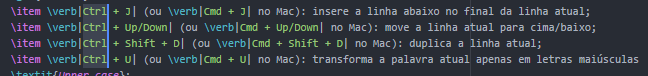
\includegraphics[scale = 0.8]{multcursor}
		\caption{Recurso de múltilplos cursores pala selecionar a palavra "Ctrl".}
	\end{figure}

	Esta funcionalidade pode ser extremamente útil para tarefas repetitivas, como renomear variáveis ou alterar o formato de algum texto. É possível também usar a seleção do mouse com a tecla \verb|Ctrl| (ou \verb|Cmd| no Mac) para selecionar outras regiões simultaneamente.

	\subsubsection{Regiões}
	Atom lida com regiões de maneira inteligente. A aparência dos limitadores\footnote{Entende-se por limitadores as maneiras tradicionais de delimitar regiões: \verb*|[]|, \verb*|()| e \verb*|{}|.} é, de fato, dada pelo destque de sintaxe a que está submetido.  Contudo, o Atom autocompleta os limitadores, \verb|""|, \verb|''| e \verb|<>| (caso a sintaxe suporte). Além disso, o Atom oferece alguns atalhos para navegar entre as regiões:
	\begin{itemize}
		\item \verb|Ctrl + M| Avança para o limitador que faz par com o atual;
		\item \verb|Alt + Ctrl + ,| (\verb|Cmd + Ctrl + M| no Mac) Seleciona todo o texto entre os limitadores que o cursor se encontra;
		\item \verb|Alt + Ctrl + .| (\verb|Alt + Cmd + .| no Mac) fecha a atual tag XML/HTML;
	\end{itemize}

	Essa funcionalidade é implementada pelo pacote de limitador chamado \verb|bracket-matcher|, cuja documentação é encontrada em \href{https://github.com/atom/bracket-matcher}{https://github.com/atom/bracket-matcher}.

	\section{Hackeando o Atom}
	Aqui existem inúmeros tópicos a respeito de orientar o usuário de forma instrutiva a desevolver seus próprios pacotes, funcionalidades e customizações diversas do Atom. Contudo, estas informações não serão abordadas aqui visto que o escopo do artigo contempla apenas a parte introdutória e de essencial entendimento. Contudo, grande parte das informações aqui omitidas podem ser encontradas em \href{https://flight-manual.atom.io/hacking-atom}{https://flight-manual.atom.io/hacking-atom}.

	Este trecho pode requerer determinado conhecimento a respeito de tecnologias específicas.

	\subsection{Hackeando o Núcleo do Atom} \label{sec:hackingcore}
	Se um usuário por acaso encontrar algum \textit{bug} no Atom ou apenas queira experimentar uma determinada funcionalidade particular do núcleo ou do sistema, é possível executar o Atom em Modo Desenvolvedor (com mais explanações na Seção \ref{sec:dev}) com acesso a uma cópia local do código-fonte do Atom.

	Basta executar um \textit{fork} (instruções em \href{https://help.github.com/articles/fork-a-repo/}{https://help.github.com/articles/fork-a-repo/}) no repositório oficial do Atom para ter acesso local ao código-fonte. Feito isso, basta clonar o repositório que foi ramificado para o repositório local, o que pode ser feito através da linha de comando:
	\begin{Verbatim}[fontsize=\footnotesize]
$ git clone git@github.com:nomeusuario/atom.git
	\end{Verbatim}
	onde \verb|nomeusuario| é o Nome de Usuário do usuário.

	Dentro do diretório clonado, pode-se instlar as dependências necessárias através da seguinte linha de comando:
\begin{Verbatim}[fontsize=\footnotesize]
$ script/bootstrap
\end{Verbatim}
	válida para todos os Sistemas Operacionais.

	\subsubsection{Modo Desenvolvedor}\label{sec:dev}
	Dado um repositório local com o código-fonte do Atom e executado o \textit{script} de \textit{bootstrap} para instalar as dependências, pode-se executar o Atom em Modo Desenvolvedor (doravante chamado Dev Mode). Antes de tudo, deve-se criar uma variável de ambiente do Sistema Operacional denominada \verb|ATOM_DEV_RESOURCE_PATH| que apontará para o diretório clonado. Feito isso, basta, em qualquer sistema operacional, inserir a seguinte linha de comando:
\begin{Verbatim}[fontsize=\footnotesize]
$ atom --dev pasta
\end{Verbatim}
	onde \verb|pasta| é um parâmetro opcional para abrir uma Pasta de Projeto.

	Existem duas vantagens principais em utilizar o Atom no Modo Desenvolvedor:
	\begin{enumerate}
		\item Se a variável \verb|ATOM_DEV_RESOURCE_PATH| for corretamente criada, o Atom estará sendo executado a partir do código-fonte local e não será mais necessário executar \verb|script/bootstrap| a cada vez que o código do Atom for alterado, bastando reiniciá-lo.
		\item Pacotes já existentes na pasta \verb|.atom| são carregados em vez dos que estão em outros locais (ainda que com mesmo nome), o que significa que o usuário pode desenvolver versões dos pacotes localmente e, facilmente, retornar a versões estáveis executando o Atom fora do Dev Mode.
	\end{enumerate}

	\subsubsection{Executando Testes Localmente}
	Para executar os testes no Núcleo do Atom a partir do terminal, deve-se primeiramente verificar se a variável \verb|ATOM_DEV_RESOURCE_PATH| explanada na Seção \ref{sec:dev} está criada. Feito isso, roda-se a seguinte linha de código na pasta do código-fonte local:
\begin{Verbatim}[fontsize=\footnotesize]
$ atom --test spec
\end{Verbatim}

	As instruções a seguir servem para a plataforma Linux. Para Mac e Windows, consulte \href{https://flight-manual.atom.io/hacking-atom/sections/hacking-on-atom-core/}{https://flight-manual.atom.io/hacking-atom/sections/hacking-on-atom-core/}.

	Antes de sequer iniciar, alguns requisitos devem ser atendidos:
	\begin{itemize}
		\item Deve-se possuir um Sistema Operacional com aquitetura 64 ou 32 bits;
		\item C++11 \textit{toolchain};
		\item Git;
		\item Node.js 6.0 ou superior;
		\item Verificar se o \textit{node-gyp} está utilizando \textit{python2} (comando de verificação (pode requerer autorização de administrador): \verb|npm config set python /usr/bin/python2 -g|)
		\item Bibliotecas do \textit{Libsecret}, disponíveis em \href{https://wiki.gnome.org/Projects/Libsecret}{https://wiki.gnome.org/Projects/Libsecret}.
	\end{itemize}

	A seguir serão abordados procedimentos preparatórios em algumas distribuições do Linux e, posteriormente, no parágrafo \textbf{Instruções}, serão prestadas orientações gerais para todas as distribuições.

	\paragraph{Ubuntu/Debian}
	Requer instação dOS cabeçalhos utilizados pelo GNOME:
\begin{Verbatim}[fontsize=\footnotesize]
$ sudo apt-get install build-essential git libsecret-1-dev fakeroot rpm \
  libx11-dev libxkbfile-dev
\end{Verbatim}
	Após isso, basta executar \verb|script/build|.

	Em caso de erro, pode ser necessário um compulador alternativo ao C++11:
\begin{Verbatim}[fontsize=\footnotesize]
$ sudo add-apt-repository ppa:ubuntu-toolchain-r/test
$ sudo apt-get update
$ sudo apt-get install gcc-5 g++-5
$ sudo update-alternatives --install /usr/bin/gcc gcc /usr/bin/gcc-5 80 \
  --slave /usr/bin/g++ g++ /usr/bin/g++-5
$ sudo update-alternatives --config gcc # choose gcc-5 from the list
\end{Verbatim}

	\paragraph{Fedora / CentOS / RHEL}
	Basta executar
	\begin{Verbatim}[fontsize=\footnotesize]
$ sudo yum install -y make gcc gcc-c++ glibc-devel git-core libsecret-devel \
  rpmdevtools
	\end{Verbatim}

	\paragraph{Arch}
	Primeiramente executa-se \verb|export PYTHON=/usr/bin/python2| e, então, executa-se:
	\begin{Verbatim}[fontsize=\footnotesize]
$ sudo pacman -S --needed gconf base-devel git nodejs npm libsecret python2 \
  libx11 libxkbfile
	\end{Verbatim}

	\paragraph{Slackware}
	Basta executar
	\begin{Verbatim}[fontsize=\footnotesize]
$ sbopkg -k -i node -i atom
	\end{Verbatim}

	\paragraph{openSUSE}
	Basta executar
	\begin{Verbatim}[fontsize=\footnotesize]
$ sudo zypper install nodejs nodejs-devel make gcc gcc-c++ glibc-devel git-core \
  libsecret-devel rpmdevtools libX11-devel libxkbfile-devel
	\end{Verbatim}

	\paragraph{Instruções}
	Feito isso, basta executar:
	\begin{Verbatim}[fontsize=\footnotesize]
$ script/build
	\end{Verbatim}
	Pode-se utilizar os seguintes parâmetros:
	\begin{itemize}
		\item \verb|--compress-artifacts| : compacta a aplicação em \verb|out/atom-{arch}.tar.gz|
		\item \verb|--create-debian-package| : cria um pacote \textit{.deb} em \verb|out/atom-{arch}.deb|
		\item \verb|--create-rpm-package| : cria um pacote \textit{.rpm} em \verb|out/atom-{arch}.rpm|
		\item \verb|--install[=dir]| : instala a aplicação em \verb|${dir}|, onde por padrão \verb|${dir} = /usr/local|
	\end{itemize}

	\bibliographystyle{sbc}
	\bibliography{references}

\end{document}
